\enteteExam{NFP 107 -- Systèmes de gestion de bases de données - Durée 2h30}%
{Examen du 12 juin  2024}%
{Documents autorisés\,: 5 pages recto-verso de notes manuscrites ou imprimées}%


Nous avons affaire à une base de données décrivant les concerts d'un festival.
Voici le schéma 
 relationnel, dans lequel les clés primaires sont en gras
(à vous de trouver les clés étrangères)\,:

\begin{itemize}
    \item Festival (\textbf{id}, nom, année)
  \item Groupe (\textbf{id}, nom, annéeFormation, nbMembres, pays)
   \item Lieu (\textbf{nom}, type, ville, capacité)
   \item Concert (\textbf{idConcert}, nomLieu, dateConcert, nbBilletsVendus, idFestival)
   \item Participation (\textbf{idConcert, idGroupe}, position)
\end{itemize}

Pour un groupe sont stockés son nom, l'année où 
l'artiste/le groupe a débuté, le nombre de membres 
composant le groupe (1 pour un artiste en solo) et son pays d'origine.

Les concerts sont donnés par un ou plusieurs groupes qui se succèdent sur scène.
La table \texttt{Participation} indique quel groupe a participé à quel concert et en quelle position.
Les concerts se déroulent dans un lieu, ont lieu à une date 
et ont un nombre de billets vendus. 

Pour le lieu nous connaissons son nom, 
son type (stade, arène, champ, église, etc), 
sa ville et son nombre de places. 

\section{Conception (6 points)}

\begin{enumerate}

\item Donnez les commandes SQL de création des tables \texttt{Concert}, \texttt{Lieu}
    et \texttt{Participation}. 

   \item Donnez le schéma conceptuel (entité / association) de cette base

    \item Un groupe peut-il participer à deux concerts différents d'un même festival (expliquer)?
    \item Un groupe peut-il jouer deux fois dans un même concert (à des positions différentes)?
 
    \item La plupart des festivals sont récurrents et proposent 
     une nouvelle édition chaque année. Une révision de la conception
     permet d'identifier les dépendances fonctionnelles suivantes\,:
     \begin{itemize}
       \item $idFestival \to nom $
       \item $idFestival, ann\acute{e}e \to directeur, budget$
     \end{itemize}
     Quel est l'impact sur le schéma relationnel\,? A-t-on de 
     nouvelles tables (dans ce cas indiquer clés primaire et étrangères) 
     et quelles modifications
     sont nécessaires sur les tables existantes\,?
     
    \item Sur le schéma obtenu, quelles tables résultent d'une
    association plusieurs-plusieurs, quelles tables 
    résultent d'une entité faible (expliquer)
\end{enumerate}

\begin{solution}

\begin{enumerate}
\item
\begin{minted}{sql}
create table Concert(
    idConcert int not null,
    nomLieu varchar(50)
    dateConcert date,
    nbBilletsVendus int,
    primary key (idConcert),
    foreign key (nomLieu) references Lieu(nom))
\end{minted}

\item Voir la figure\,\ref{concert}.

\begin{center}
  \begin{figure}[htb]  
   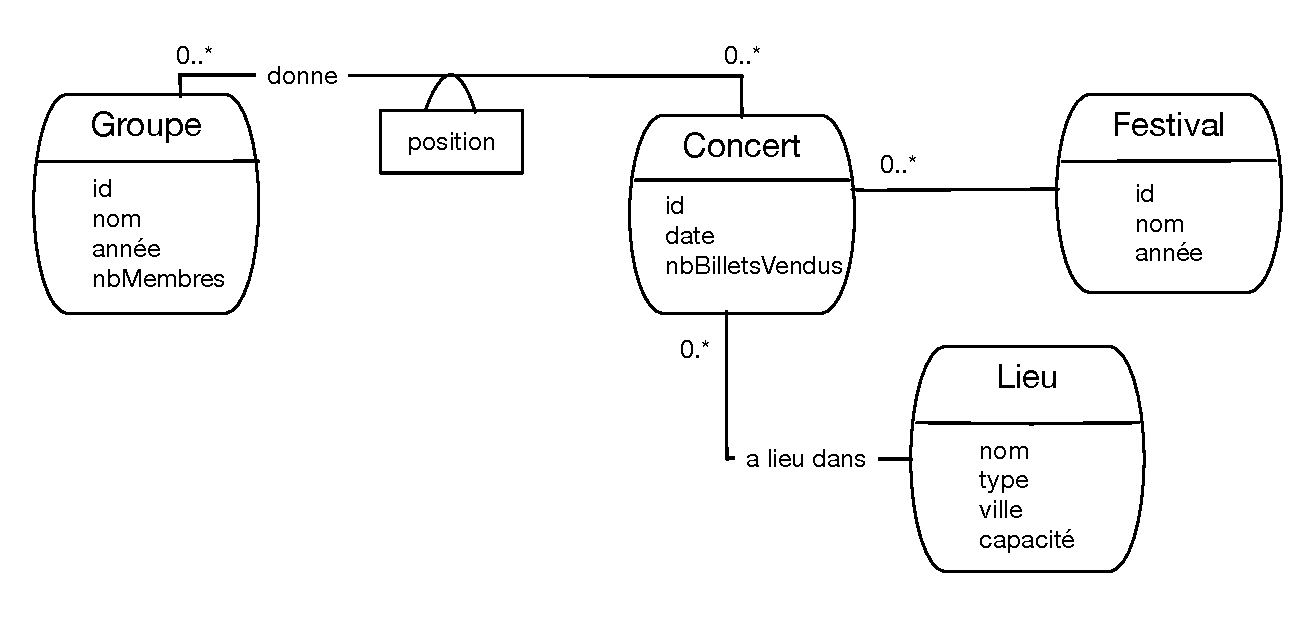
\includegraphics[scale=0.6]{../supports/figures/exam-19-concerts}
    \caption{Modélisation de la base des concerts}  
    \label{concert}  
  \end{figure}  
\end{center}


    \item Oui, un groupe peut participer à deux concerts différents: la clé composite
        de la table \texttt{Participation} le permet.
    \item Un groupe peut-il jouer deux fois dans un même concert : non car position ne fait
    pas partie de la clé
 
    \item On applique l'algorithme de normalisation.
    On doit retirer l'année de la table \texttt{Festival} 
    qui devient  Festival (\textbf{id}, nom). On ajoute 
    une table \'Edition (\textbf{\textit{idFestival}, année}, directeur, budget).
    
    Enfin, en bonus, il faut sans doute changer la clé étrangère dans la table
    Concert pour référencer une édition avec la paire (idFestival, année)
    
    \item Participation vient d'une association plusieurs-plusieurs, 
    tandis que \'Edition est une entité faible (on ne peut 
    pas avoir d'édition dans festival).
\end{enumerate}
\end{solution}


\section{SQL (8 points)}

Les requêtes s'expriment sur le schéma \emph{donné dans l'énoncé} (avant 
donc l'introduction les évolutions liées à la notion d'édition).

\begin{enumerate}

\item Quels lieux ont servi au festival de Woodstock en 1969?

\begin{solution}
\begin{minted}{sql}
select c.nomLieu
from Concert as c, Festival as f
where c.idFestival=f.id
and f.nom='Woodstock'
and f.année = 1969
\end{minted}
\end{solution}

\item Combien de billets ont été vendus pour le concert auquel ont participé les \textit{Who}
(c'est un nom de groupe...) à Woodstock en 1969?

\begin{solution}
\begin{minted}{sql}
select c.nbBilletsVendus
from Concert as c, Festival as f, Participation as p, Groupe as g
where c.idFestival=f.id
and  p.idConcert=c.id
and p. idGroupe=g.id
and g.nom='Who'
and f.nom='Woodstock'
and f.année = 1969
\end{minted}
\end{solution}

\item Donnez les noms des groupes qui n'ont pas participé à Woodstock 1969

\begin{solution}
\begin{minted}{sql}
select g.nom
from Groupe as g
where not exists (select *
        from Concert as c, Festival as f, Participation as p
        where c.idFestival=f.id
        and  p.idConcert=c.id
        and p.idGroupe=g.id
        and f.nom='Woodstock'
        and f.année = 1969)
\end{minted}
\end{solution}


\item Combien de concerts ont été donnés par les Beatles  
(c'est un nom de groupe\,!) à Paris
(c'est un nom de ville\,!)

\begin{solution}
\begin{minted}{sql}
select count(*)
from Groupe as g, Concert as c, Participation as p, Lieu as l
where p.idConcert=c.id
and p.idGroupe=g.id
and c.nomLieu = l.nom
and.ville = 'Paris'
and g.nom='Beatles'
\end{minted}
\end{solution}

\item Pour chaque concert donnez le nom du groupe ayant joué en dernière position (affichez l'id du concert
et le nom du groupe).

\begin{solution}
\begin{minted}{sql}
select c.idConcert, g.nom
from Groupe as g, Concert as c, Participation as p1
where p.idConcert=c.id
and p. idGroupe=g.id
and not exists = (select * 
                  from Participation as p2 
                  where p2.idConcert=c.id
                  and p1. position <= p2.position)
\end{minted}
\end{solution}


\item Quels groupes ont joué plusieurs fois dans un même festival (affichez le nom
du festival, le nom du groupe, et le nombre de participations).

\begin{solution}
\begin{minted}{sql}
select f.nom as nomFestival, g.nom as nomGroupe, count(*) as nbPart
from Festival as f, Groupe as g, Concert as c, Participation as p
where p.idConcert=c.id
and p. idGroupe=g.id
and c.idfestival = f.id
group by g.id, f.id, g.nom, f.nom
having count(*) > 1
\end{minted}
\end{solution}
\end{enumerate}


\section{Algèbre (3 points)}

\begin{enumerate}
   \item Donnez l'expression algébrique pour la première requête SQL (section précédente)

   \item Expliquez le sens de l'expression algébrique suivante, puis   
  donnez la requête SQL correspondante.
  \item 
       $$\pi_{nom} (Lieu) - \pi_{nomLieu} (Concert)$$

\end{enumerate}


\begin{solution}

\begin{enumerate}
\item $\pi_{nomLieu} (\sigma_{nom='Woodstock' \land annee=1969} (Festival) \Join_{id=idFestival} Concert)$ 

   \item Les lieux où aucun concert n'a eu lieu.


\begin{minted}{sql}
select nom
from Lieu 
where nom not in (select nomLieu from Concert)
\end{minted}
\end{enumerate}

\end{solution}


  
\section{Normalisation ({\bf 3 pts})}

On considère une table \texttt{idC,idG,position,nomLieu,nomGroupe} avec
les dépendances fonctionnelles: $idC \to nomLieu$, $idG \to nomGroupe$ et
$idC, idG \to position$.

\begin{enumerate}
   \item Quelle est la clé\,?
   \item Montrez que cette table n'est pas en troisième forme normale
   \item Quel est le schéma résultant de la normalisation.
   
\end{enumerate}
\begin{solution}
   \begin{enumerate}
      \item La clé est (idC, idG)
       \item Non à cause de $idC \to nomLieu$, ainsi que $idG \to nomGroupe$
       \item On obtient le schéma de l'énoncé
    \end{enumerate}
\end{solution}

